\section{小波刻画}
\label{sec:besov-wavelet}

差分范数直接表达了“尺度$t$上的变化”，但用它计算逼近误差并不方便：误差要求知道函数由哪些成分组成，连续模只给出整体的变化量。小波基给出函数的坐标，第$j$层系数正好对应尺度$2^{-j}$附近、不同位置上的变化。本节把差分范数改写成对坐标的条件，后面三节都在这组坐标中计算。

\paragraph{周期小波基与系数}
由第~\ref{chap:wavelet-transform}章，取实值的紧支撑正交多分辨率分析，尺度函数$\varphi$与母小波$\psi$都支撑在$[0,L]$中，令$\varphi_{j,k}(x)=2^{j/2}\varphi(2^jx-k)$，$\psi_{j,k}$同理，再沿整数平移求和得到周期基函数。为简洁，本章省去周期化的上标。

固定起始尺度$j_0\geq0$，并要求$2^{j_0}\geq L$，使每个$\psi_{j,k}$（$j\geq j_0$）的支撑在一个周期内不与自身的平移重叠。由第~\ref{chap:wavelet-transform}章的周期小波基定理，下面的函数族是$L^2(\mathbb T)$的标准正交基：
\[
 \{\varphi_{j_0,k}:0\leq k<2^{j_0}\}\cup\{\psi_{j,k}:j\geq j_0,\ 0\leq k<2^j\}.
\]

基函数有界，所以对$f\in L^p(\mathbb T)\subset L^1(\mathbb T)$可以用积分读取系数。粗项系数记为$a_k$，第$j$层细节系数记为$c_{j,k}$：
\[
 a_k=\int_0^1f\varphi_{j_0,k},\qquad c_{j,k}=\int_0^1f\psi_{j,k} .
\]
记$a=(a_k)_{0\leq k<2^{j_0}}$，$c_j=(c_{j,k})_{0\leq k<2^j}$。对$f\in L^2(\mathbb T)$，Parseval等式给出
\[
 \lVert f\rVert_2^2=\lVert a\rVert_{\ell^2}^2+\sum_{j\geq j_0}\lVert c_j\rVert_{\ell^2}^2 .
\]

这样每个函数就对应一个分组的无限维向量$[a\mid c_{j_0}\mid c_{j_0+1}\mid\cdots]$，第$j$组有$2^j$个分量。

\paragraph{贯穿后文的例子}
后面三节用一个能手算的函数：$f=\mathbf 1_{[0,1/3)}$按周期$1$延拓，用Haar基，$j_0=0$，$a_0=\int_0^1f=1/3$。跳跃点$1/3$不在任何二进分点上，这正是选它的原因；若跳在$1/2$，Haar展开只有一项，不具代表性。周期平移差与上一节相同，当$\lvert h\rvert\leq1/3$时$\lVert\Delta_hf\rVert_2=(2\lvert h\rvert)^{1/2}$。

计算第$j$层的系数。若$\psi_{j,k}$的支撑不含$1/3$，则$f$在支撑上是常数，由$\int\psi_{j,k}=0$可知系数为零。所以每层只有一个非零系数，位于$k_j=\lfloor2^j/3\rfloor$。令$\theta=2^j/3-k_j$，则$j$为偶数时$\theta=1/3$，$j$为奇数时$\theta=2/3$。

在这个区间上，$f$只在相对位置$[0,\theta)$上等于$1$。$\psi_{j,k_j}$在左半取值$2^{j/2}$、右半取值$-2^{j/2}$，区间长度为$2^{-j}$，所以
\[
 c_{j,k_j}=2^{-j/2}\Bigl(\int_0^\theta\mathbf 1_{[0,1/2)}-\int_0^\theta\mathbf 1_{[1/2,1)}\Bigr)=\frac{2^{-j/2}}{3},
\]
$\theta=1/3$时括号内是$1/3$，$\theta=2/3$时括号内是$1/2-1/6=1/3$。

用Parseval等式核对：坐标的平方和为
\[
 \frac19+\sum_{j\geq0}\frac{2^{-j}}{9}=\frac19+\frac29=\frac13=\lVert f\rVert_2^2 .
\]

\subsection{单尺度系数的大小}
\label{sec:besov-single-scale}

先看一组坐标怎样对应函数的大小。$\psi_{j,k}$在$L^2$中归一化，其$L^p$范数却随尺度变化。换元$y=2^jx-k$给出
\begin{equation}
 \lVert\psi_{j,k}\rVert_p=2^{j/2}\Bigl(\int\lvert\psi(2^jx-k)\rvert^p\,\mathrm dx\Bigr)^{1/p}=2^{j(1/2-1/p)}\lVert\psi\rVert_p .
 \label{eq:besov-psi-lp}
\end{equation}
$p=2$时因子为$1$；$p<2$时细尺度上单个小波的$L^p$范数变小，$p>2$时变大。这是$L^2$归一化与$L^p$度量之间的换算，与函数的光滑性无关。

同一层的小波支撑长度为$L2^{-j}$，每点至多被有限个支撑覆盖，所以一层的组合大致是这些“块”的不交拼接，其$L^p$范数应当与单块范数乘以系数的$\ell^p$范数相当。这正是分组向量的“组内$\ell^p$”的来源。

\begin{lemma}[单层组合的$L^p$大小]
\label{lem:besov-single-level}
设$1\leq p\leq\infty$，$j\geq j_0$。存在只依赖$\psi$、$L$与$p$的常数$0<c\leq C$，使对任意系数$(c_k)_{0\leq k<2^j}$，函数$g=\sum_kc_k\psi_{j,k}$满足
\begin{equation}
 c\,2^{j(1/2-1/p)}\lVert(c_k)\rVert_{\ell^p}\leq\lVert g\rVert_p\leq C\,2^{j(1/2-1/p)}\lVert(c_k)\rVert_{\ell^p} .
 \label{eq:besov-single-level}
\end{equation}
\end{lemma}

\begin{proof}
记$m=\lceil L\rceil+1$，每点至多属于$m$个支撑$I_k=\operatorname{supp}\psi_{j,k}$。先设$p<\infty$。

上界：在每点只有至多$m$个非零项，由有限和的Hölder不等式，
\[
 \lvert g(x)\rvert^p\leq m^{p-1}\sum_k\lvert c_k\rvert^p\lvert\psi_{j,k}(x)\rvert^p .
\]
积分后用式~\eqref{eq:besov-psi-lp}，得到
\[
 \lVert g\rVert_p^p\leq m^{p-1}\lVert\psi\rVert_p^p\,2^{j(p/2-1)}\sum_k\lvert c_k\rvert^p .
\]

下界：由正交性，$c_k=\int_{I_k}g\psi_{j,k}$。记$p'$为$p$的共轭指数，Hölder不等式给出
\[
 \lvert c_k\rvert\leq\lVert g\rVert_{L^p(I_k)}\lVert\psi_{j,k}\rVert_{p'}=\lVert g\rVert_{L^p(I_k)}\,2^{j(1/p-1/2)}\lVert\psi\rVert_{p'}.
\]

取$p$次方后对$k$求和，每点至多被计入$m$次，于是
\[
 \sum_k\lvert c_k\rvert^p\leq m\,2^{j(1-p/2)}\lVert\psi\rVert_{p'}^p\lVert g\rVert_p^p.
\]
两边开$p$次方，就是所要的下界。$p=\infty$时把求和换成最大值，论证相同。
\end{proof}

上界只用到支撑的重叠次数和$\psi$有界，把$\psi$换成其他紧支撑有界函数仍然成立，下一小节要用这一点。

\paragraph{手算：集中与分散}
对Haar小波，同层支撑两两不交，$\lvert\psi_{j,k}\rvert$在支撑上恒为$2^{j/2}$，式~\eqref{eq:besov-single-level}两端恰好相等。取$j=3$，比较两组$\ell^2$范数都是$1$的系数：
\[
 c^{\mathrm A}=(1,0,\ldots,0),\qquad c^{\mathrm B}=\frac{1}{\sqrt8}(1,\ldots,1).
\]

$c^{\mathrm A}$的能量集中在一个位置，对应的函数是高为$2^{3/2}$的窄脉冲。$c^{\mathrm B}$的能量分散到全部$8$个位置，对应的函数在每点取值$\pm1$。把它们的组内范数代入式~\eqref{eq:besov-single-level}，结果列在表~\ref{tab:besov-concentrate-spread}中。

\begin{BookInlineTable}
  \centering
  \begin{tabular}{@{}llll@{}}
    \toprule
    & $p=1$ & $p=2$ & $p=\infty$\\
    \midrule
    因子$2^{3(1/2-1/p)}$ & $2^{-3/2}$ & $1$ & $2^{3/2}$\\
    $\lVert c^{\mathrm A}\rVert_{\ell^p}$ & $1$ & $1$ & $1$\\
    $\lVert c^{\mathrm B}\rVert_{\ell^p}$ & $2^{3/2}$ & $1$ & $2^{-3/2}$\\
    $\lVert g^{\mathrm A}\rVert_p$ & $0.354$ & $1$ & $2.83$\\
    $\lVert g^{\mathrm B}\rVert_p$ & $1$ & $1$ & $1$\\
    \bottomrule
  \end{tabular}
  \caption{同一层上两组系数的$L^p$大小。集中的系数在$p$较大时显得大，分散的系数对各个$p$相同。}
  \label{tab:besov-concentrate-spread}
\end{BookInlineTable}

\begin{BookInlineFigure}
  \centering
  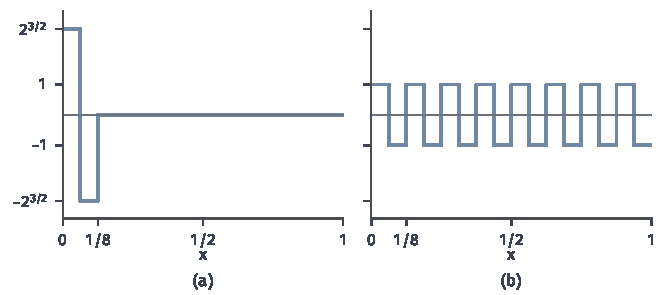
\includegraphics[width=112mm]{figures/04-spaces-measures-and-geometry/03-function-spaces/matplotlib/besov-lp-position/figure.pdf}
  \caption{第$3$层Haar组合。(a)系数集中：$g^{\mathrm A}=\psi_{3,0}$，是一个高$2^{3/2}$、宽$1/8$的脉冲。(b)系数分散：$g^{\mathrm B}=8^{-1/2}\sum_k\psi_{3,k}$，处处$\lvert g^{\mathrm B}\rvert=1$。两者系数的$\ell^2$范数相同。}
  \label{fig:besov-lp-position}
\end{BookInlineFigure}

图~\ref{fig:besov-lp-position}解释了这张表。$L^2$看不出区别，$L^\infty$只看峰值，脉冲因此显得大，$L^1$看总面积，脉冲因此显得小。$2^{j(1/2-1/p)}\lVert c_j\rVert_{\ell^p}$正是第$j$层细节在$L^p$中的大小，$\ell^p$范数把差分范数中“同一尺度、不同位置”的汇总搬到了坐标上。

再乘以$2^{js}$，就把这一层的大小与期望量级$2^{-js}$相比较，对应差分范数中的$t^{-s}$。粗项$a$只有$2^{j_0}$个分量，记录最大尺度上的整体大小，对应差分范数中的$\lVert f\rVert_p$；它不能省略，否则常数函数会得到零范数。

\subsection{小波等价范数}
\label{sec:besov-wavelet-norm}

把上述加权块大小按$\ell^q$汇总，就得到候选的系数范数。记
\begin{equation}
 b_j=2^{j(s+1/2-1/p)}\lVert c_j\rVert_{\ell^p},\qquad j\geq j_0 ,
 \label{eq:besov-block}
\end{equation}
并令
\begin{equation}
 \lVert f\rVert_{B^s_{p,q}}^{\mathrm w}=\lVert a\rVert_{\ell^p}+\bigl\lVert(b_j)_{j\geq j_0}\bigr\rVert_{\ell^q},
 \label{eq:besov-wavelet-norm}
\end{equation}
其中$q=\infty$时取上确界。

图~\ref{fig:besov-group-coordinates}是这个范数的计算过程。它与有限维的分组范数只有两点不同：组数无穷，组的长度$2^j$随下标增长。权重中的$s$体现光滑性要求，$1/2-1/p$只是归一化换算。

\begin{BookInlineFigure}
  \centering
  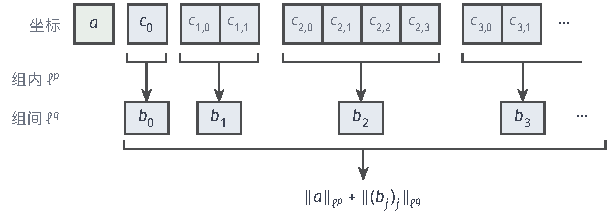
\includegraphics[width=103.3mm]{figures/04-spaces-measures-and-geometry/03-function-spaces/tikz/besov-group-coordinates/figure.pdf}
  \caption{Besov范数是分组加权的向量范数（图中取$j_0=0$）。第一行是函数的小波坐标，蓝色方格按尺度分组，第$j$组有$2^j$个分量，绿色方格是粗项。第二行把每组用$\ell^p$范数合成一个数，并乘以权重，得到式~\eqref{eq:besov-block}的$b_j$。最后对各组的$b_j$取$\ell^q$范数，再加上粗项。}
  \label{fig:besov-group-coordinates}
\end{BookInlineFigure}

用贯穿的例子算一次。取$p=2$、$q=2$、$s=1/4$，此时权重为$2^{j/4}$，每组只有一个非零坐标，所以
\[
 b_j=2^{j/4}\cdot\frac{2^{-j/2}}{3}=\frac{2^{-j/4}}{3}.
\]
前几项约为$0.333$、$0.280$、$0.236$、$0.198$。

对$b_j^2$求几何和，再加上粗项，得到
\[
 \lVert(b_j)\rVert_{\ell^2}^2=\frac{1/9}{1-2^{-1/2}}\approx0.3794,\qquad\lVert f\rVert^{\mathrm w}_{B^{1/4}_{2,2}}=\frac13+\sqrt{0.3794}\approx0.949 .
\]
若取$s=1/2$，则$b_j=1/3$对所有$j$成立，序列有界而不可和，与差分计算得到的式~\eqref{eq:besov-step-membership}一致。

\begin{theorem}[小波刻画]
\label{thm:besov-wavelet-characterization}
设$1\leq p,q\leq\infty$，$s>0$。设$\varphi$与$\psi$有直到$m$阶的连续导数且$m>s$，$\psi$有$M>s$个消失矩，即$\int x^i\psi(x)\,\mathrm dx=0$对$0\leq i<M$成立，$m$与$M$为整数。则存在常数$C_0\geq1$，使对每个$f\in L^p(\mathbb T)$，
\begin{equation}
 C_0^{-1}\lVert f\rVert_{B^s_{p,q}}^{\mathrm w}\leq\lVert f\rVert_{B^s_{p,q}}\leq C_0\lVert f\rVert_{B^s_{p,q}}^{\mathrm w},
 \label{eq:besov-wavelet-equivalence}
\end{equation}
两端同时有限或同时无限。$C_0$依赖$s,p,q$、所选小波与$j_0$。
\end{theorem}

下面写出证明的主要步骤，并分开说明两个方向分别依赖小波的哪种性质。证明中有三处引用外部事实：差分范数不依赖$r$，一般$r$的局部多项式逼近估计，以及$p<2$时小波展开在$L^p$中的收敛。取$r=\lfloor s\rfloor+1$，由$m,M$是大于$s$的整数，得到$s<r\leq\min(m,M)$。记
\[
 g_j=\sum_kc_{j,k}\psi_{j,k},\quad B_j=2^{j(1/2-1/p)}\lVert c_j\rVert_{\ell^p},\quad b_j=2^{js}B_j .
\]

\paragraph{由系数控制差分：正则性}
设系数范数有限。由引理~\ref{lem:besov-single-level}，$\lVert g_j\rVert_p\leq CB_j=C2^{-js}b_j$，而$(b_j)$有界，所以$\sum_jg_j$在$L^p$中绝对收敛，它的系数就是$f$的系数。系数全为零的$L^p$函数只有零：$p\geq2$时这是$L^2$基的完备性，$p<2$时需要用尺度函数核的估计说明投影$P_J$在$L^p$上一致有界。于是$f$等于这个级数。

对单层作差分。小步长用导数，大步长用$2^r$。$g_j^{(r)}$是由$2^{jr}(\psi^{(r)})_{j,k}$组合成的，由引理证明的上界部分，有$\lVert g_j^{(r)}\rVert_p\leq C2^{jr}B_j$。代入式~\eqref{eq:besov-difference-bounds}，得到
\[
 \lVert\Delta_h^rg_j\rVert_p\leq C\min\bigl(1,(2^j\lvert h\rvert)^r\bigr)B_j .
\]

粗项同理，只是因子$2^{jr}$换成常数。对$\lvert h\rvert\leq2^{-J}$求和，把$j<J$与$j\geq J$分开：
\[
 \omega_r(f,2^{-J})_p\leq C\Bigl(2^{-Jr}\lVert a\rVert_{\ell^p}+\sum_{j<J}2^{(j-J)r}B_j+\sum_{j\geq J}B_j\Bigr).
\]

两边乘以$2^{Js}$。用$B_j=2^{-js}b_j$改写，得到
\[
 \begin{aligned}
 2^{Js}\omega_r(f,2^{-J})_p\leq C\Bigl(&2^{-J(r-s)}\lVert a\rVert_{\ell^p}\\
 &+\sum_{j<J}2^{-(J-j)(r-s)}b_j+\sum_{j\geq J}2^{-(j-J)s}b_j\Bigr).
 \end{aligned}
\]

右端是序列$(b_j)$与一个几何衰减序列的卷积。对卷积用$\ell^q$的Minkowski不等式：若$e_J\leq\sum_n\kappa_nb_{J+n}$，$\kappa_n\geq0$，则
\begin{equation}
 \lVert(e_J)\rVert_{\ell^q}\leq\Bigl(\sum_n\kappa_n\Bigr)\lVert(b_j)\rVert_{\ell^q}.
 \label{eq:besov-convolution}
\end{equation}

这里两侧的几何比是$2^{-(r-s)}$和$2^{-s}$，两者都小于$1$，恰好需要$0<s<r$。所以序列$(2^{Js}\omega_r(f,2^{-J})_p)_{J\geq j_0}$的$\ell^q$范数不超过$C(\lVert a\rVert_{\ell^p}+\lVert(b_j)\rVert_{\ell^q})$。$J<j_0$只有有限项，每项不超过$2^r\lVert f\rVert_p$。再代入式~\eqref{eq:besov-dyadic-form}，就得到式~\eqref{eq:besov-wavelet-equivalence}的右半部分。

\paragraph{由差分控制系数：消失矩}
设$\lVert f\rVert_{B^s_{p,q}}<\infty$。先写出通用的一步。把$f$看成实轴上的周期函数，由第~\ref{chap:wavelet-transform}章的展开公式，$c_{j,k}=\int_{\mathbb R}f\psi_{j,k}$，积分区域是实轴上的支撑$I_k$，长度$\delta=L2^{-j}$。因此消失矩可以在实轴上使用，无需担心跨周期接缝。

对次数小于$r\leq M$的多项式$P_k$，有$\int P_k\psi_{j,k}=0$。于是
\[
 c_{j,k}=\int_{I_k}(f-P_k)\psi_{j,k} .
\]
用Hölder不等式与式~\eqref{eq:besov-psi-lp}，再按$k$求和，得到
\[
 B_j^p\leq\lVert\psi\rVert_{p'}^p\sum_k\lVert f-P_k\rVert_{L^p(I_k)}^p .
\]

现在要选$P_k$使右端小。$r=1$时，即$0<s<1$，$P_k$取$f$在$I_k$上的平均值。由Jensen不等式，
\[
 \lvert f(x)-P_k\rvert^p\leq\frac1\delta\int_{I_k}\lvert f(x)-f(y)\rvert^p\,\mathrm dy .
\]

对$x\in I_k$积分并换元$y=x+h$，得到
\[
 \lVert f-P_k\rVert_{L^p(I_k)}^p\leq\frac1\delta\int_{\lvert h\rvert\leq\delta}\int_{I_k}\lvert\Delta_hf(x)\rvert^p\,\mathrm dx\,\mathrm dh .
\]
对$k$求和，每点至多被计入$m$次，$\mathrm dh$的积分域长度为$2\delta$，于是
\[
 \sum_k\lVert f-P_k\rVert_{L^p(I_k)}^p\leq2m\,\omega_1(f,\delta)_p^p .
\]

由$\Delta_{nh}u=\sum_{i<n}\Delta_hu(\cdot+ih)$，得到$\omega_1(f,nt)_p\leq n\,\omega_1(f,t)_p$，所以$B_j\leq C\omega_1(f,2^{-j})_p$。乘以$2^{js}$，取$\ell^q$，由式~\eqref{eq:besov-dyadic-form}，第二项受$\lVert f\rVert_{B^s_{p,q}}$控制。粗项由同样的Hölder估计得到$\lVert a\rVert_{\ell^p}\leq C\lVert f\rVert_p$。这就完成了$0<s<1$时的左半部分。$p=\infty$时把积分换成上确界，论证相同。

$r\geq2$时机制相同，平均值换成局部的最佳多项式逼近，所需的不等式是Whitney估计，它用$r$阶差分在$I_k$附近的平均控制局部多项式逼近误差，证明较长，读者可查阅逼近论的专著。没有足够的消失矩，光滑函数在细尺度上的系数就不会足够小。

\paragraph{条件不能省略}
Haar小波给出具体的反例。Haar母小波是阶跃型函数，由式~\eqref{eq:besov-step-membership}（平移与伸缩只改变常数），它在$p=2$、$s>1/2$时不属于任何$B^s_{2,q}$，在$s=1/2$时只属于$B^{1/2}_{2,\infty}$。可是在式~\eqref{eq:besov-wavelet-norm}中，单个Haar小波只有一个非零系数，系数范数有限。所以对这些参数，Haar系数范数与差分范数不可能等价。

Haar小波在$p=2$、$0<s<1/2$时仍然适用。消失矩的方向只用$r=1$，上面的证明不变。正则性的方向要改一步：第$j$层的Haar组合是网格宽度$2^{-j-1}$上的阶梯函数，$\lVert\Delta_hg_j\rVert_2$只有$(2^j\lvert h\rvert)^{1/2}$的增益，卷积的几何比变成$2^{-(1/2-s)}$，这要求$s<1/2$。这也是本章手算例子可以用Haar基的依据，手算的结果只用于$s<1/2$时的等价，$s=1/2$的端点由式~\eqref{eq:besov-step-membership}另行验证。要刻画更高的光滑阶数，必须改用更光滑、消失矩更多的小波。

下面三节固定一个满足定理~\ref{thm:besov-wavelet-characterization}条件的周期正交小波基，把差分范数与系数范数视为可以互换的度量，相差的倍数统一记入常数$C_0$。
